\chapter[Diversion Detection]{Diversion Detection}

The second aspect of this work is identifying potential places for diversion in a generic pyroprocessing facility. We took 2 primary approaches for this work, applying
a cumulative sum detection algorithm and performing sensitivity analysis on key facility parameters. 
\section{Cumulative Sum}

\subsection{Requirements of Diversion Detection}


The cumulative sum method (CUSUM) applied to Pyre was chosen to fit the following requirements: function with minimal prior information, have online diversion detection
capabilities, and fit a modular approach. The CUSUM change detection algorithm relies on developing an expected mean value of a data stream as shown by the following equations \cite{basseville_detection_1993}.

\[ f_{t+1} = max(0, f_t + x_t - \mu - \delta) \]

Where:
\[ x_t = observed \hspace{2mm} data \]
\[ \mu = approximated \hspace{2mm} mean \]
\[ \delta = acceptable \hspace{2mm} change \]

This general function adds new observed values to the calculated mean. If the value is within region of error, typically 3$\sigma$, change is not reported. 
We favor this online diversion detection capability in an effort to achieve timely detection goals set by the IAEA \cite{international_atomic_energy_agency_implications_2004}.
These intermittent inspections only have access to portions of the complete data stream, thus we aim to mimic reality as closely as possible. In addition, we need this
algorithm to work on a variety of facilities with different sub-processes active, ruling out a nodal approach seen by \cite{Yilmaz_2016}.

\subsection{Limitations of selected method}

This approach is not without its drawbacks, since there is no prior data assumed we must generate a reasonable mean before being able to detect diversion. For this work
we assume a startup time of approximately 6 months before an appropriate mean can be developed. The next limitation faced with this approach is observing one data stream at a time, while
real inspections take a wide range of conditions into account. This concern is addressed by using sensitivity analysis, as seen later in this chapter, to inform on the most crucial
sub-processes or settings. 

CUSUM relies on a variable mean and noise to obscure possible change points. When a simulator knows the exact value at each time step, without human reporting or measurement error, change 
detection becomes trivial. To combat this issue, noise is artificially created when the CUSUM class reads data. This way \Cyclus retains its constant operating value while the change point
has potential to be obscured by measurement error. These detector uncertainties are assumed from common non-destructive and destructive assay practices used by the SEE LANL course \cite{}.

\section{Verification}

\paragraph{Operator Diversion} \mbox{} \\

To test operator diversion capabilities, we ran the EG01-EG24 transition scenario shown in chapter 3 with inside operators. The scenario described in Table \ref{tab:setup} contains an LWR and SFR configuration for Pyre. Each prototype siphoned material with different quantities and frequencies to demonstrate its reconfigurability. The LWR Pyre siphoned off 5\% every 10 timesteps while the SFR Pyre siphoned off 1\% excess every other timestep.  Results for this scenario are shown in
Figure \ref{fig:divertmat}.

\begin{figure}
	\centering
	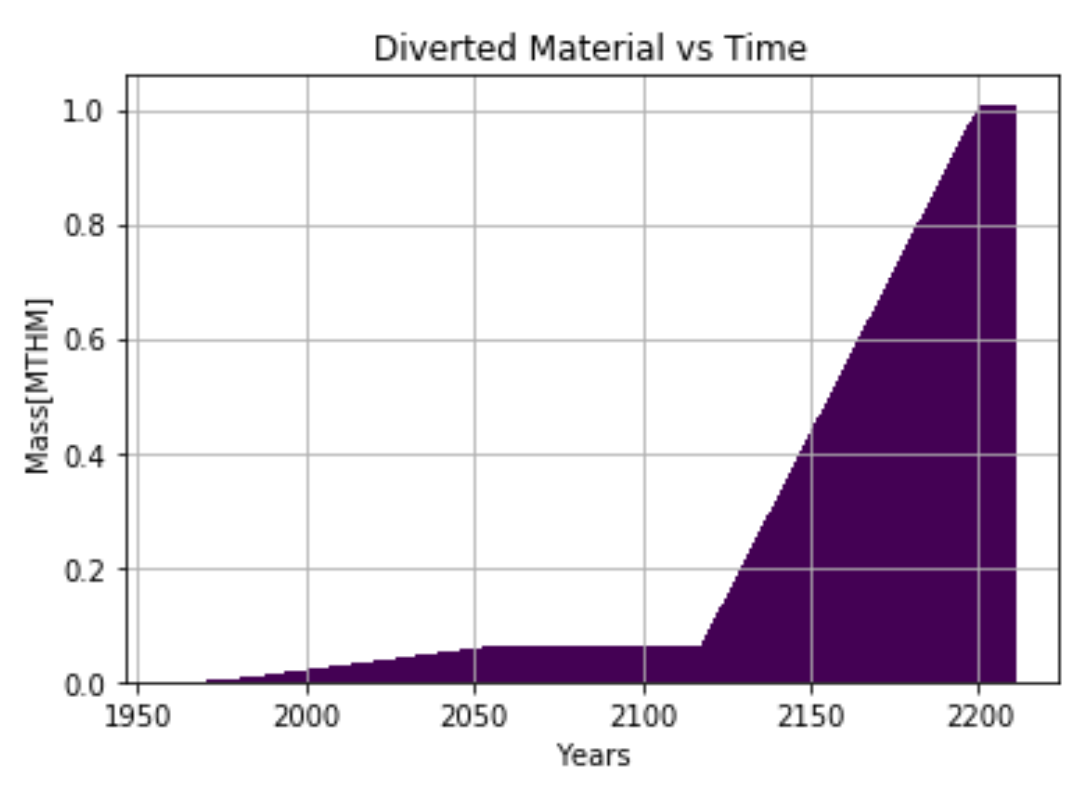
\includegraphics[width=0.9\linewidth]{images/divertmat}
	\caption{A timeseries of diverted material from two Pyre facilities.}
	\label{fig:divertmat}
\end{figure}

\section{Sensitivity Analysis}

Sensitivity analysis is an important aspect of this work to know the limits of monitoring these facilities. In this work we use Dakota to alter \Cyclus input files, allowing us to easily
run batches of scenarios. To properly use Dakota with \Cyclus, we must use DCWrapper, which uses python to interface between Dakota and \Cyclus' xml input files. 
Key parameters were run over a range of values for diversion to verify the archetype's capabilities and identify operational ranges. Parameters were selected from the most attractive
sub-processes for diversion, the electrorefiner and electrowinner. These two processes are responsible for the production of Uranium and U/TRU ingots, therefore sensitivity analysis was run
on each of their key parameters: Temperature, Current, Flowrate, Pressure, Stirrer Speed, and Reprocessing Time.

\subsection{Temperature}

The first setting for consideration is the electrorefiner's temperature. As discussed in methodology, the range for this setting is 500 to 1000 $^\circ C$. However, operation
typically occurs above 750 $^\circ C$. For each setting we observe how much material can be diverted within a month; these values can be seen isotopically in Figure \ref{fig:ref-temp-sa}.
The stream corresponding to 750 $^\circ C$ is then subtracted from remaining streams to determine the impact of increasing temperature on divertable material.
While temperature is a key aspect to the electrorefiner, Figure \ref{fig:ref-temp-diff} shows that when approaching 1000 $^\circ C$ efficiency does not increase significantly resulting
in diminishing returns.

\begin{figure}
	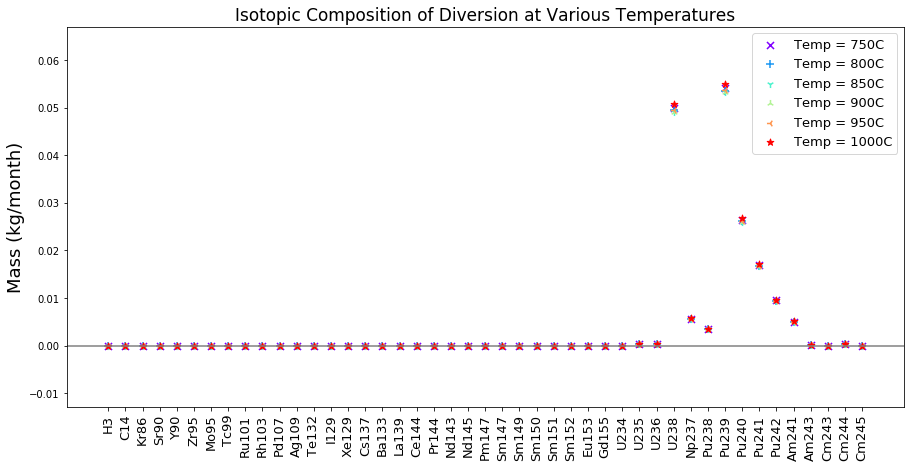
\includegraphics[width=\linewidth]{images/temperature-sa-comp}
	\caption{Isotopic composition of the Diverted material stream at various Refiner temperatures.}
	\label{fig:ref-temp-sa}
\end{figure}

\begin{figure}
	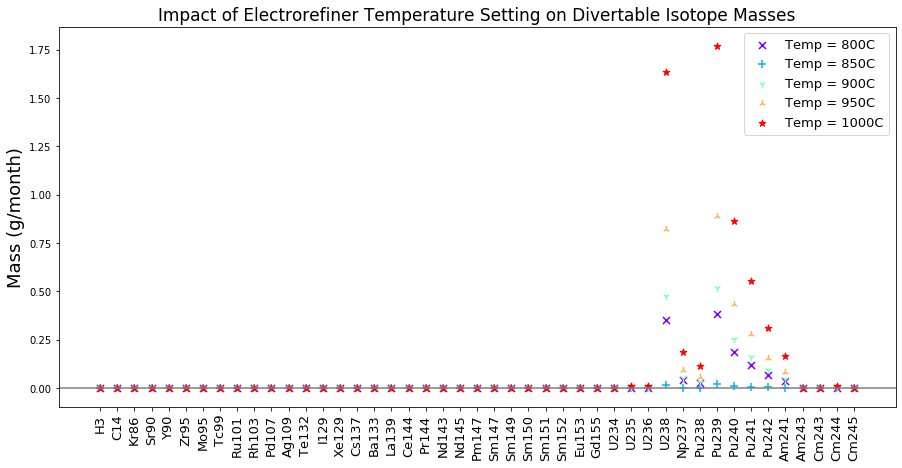
\includegraphics[width=\linewidth]{images/temperature-sa-diff}
	\caption{Isotopic composition of the Diverted material stream at various Refiner temperatures.}
	\label{fig:ref-temp-diff}
\end{figure}

\subsection{Pressure}

Available in advanced electrorefiners, vacuum pressure can improve separation efficiency as well. Similar to our analysis of temperature, isotopic compositions of
divertable material can be seen in Figure \ref{fig:ref-press-sa}. Our baseline for the comparison is atmospheric pressure as this will represent facilities lacking this
functionality. 

\begin{figure}
	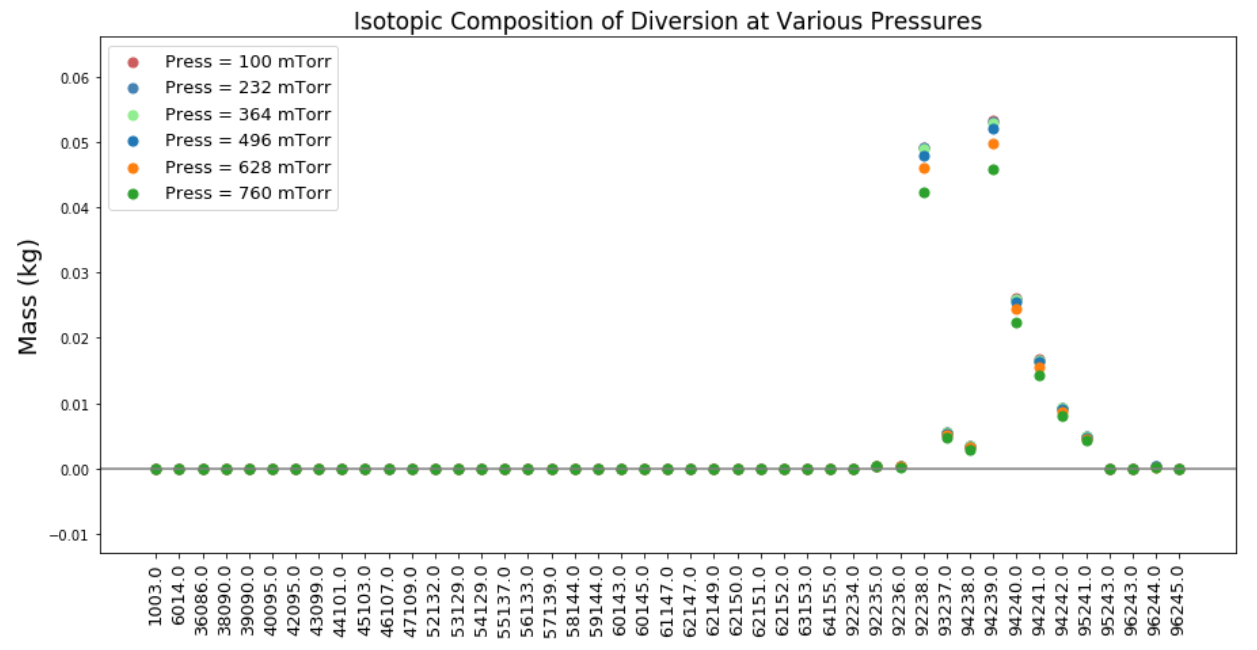
\includegraphics[width=\linewidth]{images/pressure-sa-comp}
	\caption{Isotopic composition of the Diverted material stream at various Refiner pressures.}
	\label{fig:ref-press-sa}
\end{figure}

\begin{figure}
	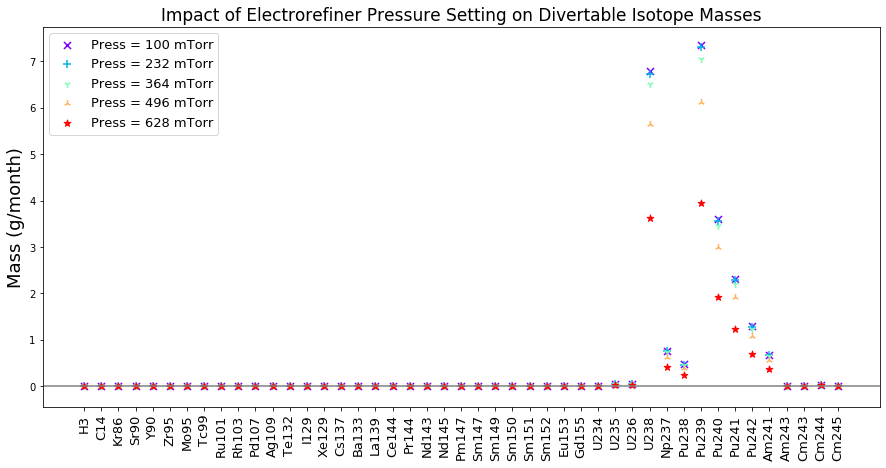
\includegraphics[width=\linewidth]{images/pressure-sa-diff}
	\caption{Isotopic composition of the Diverted material stream at various Refiner pressures.}
	\label{fig:ref-press-diff}
\end{figure}

\subsection{Stirrer Speed}

The central stirrer is another setting particular to advanced refining techniques \cite{lee_advanced_2008}. We are observing this setting as its a rather simple capability to
add a mixer. Figure \ref{fig:ref-rot-sa} shows the isotopic distribution associated with a
range of different stirrer speeds. Higher than 100 rpm results in uranium dendrites returning
to the salt. Therefore, in Figure \ref{fig:ref-rot-diff} we use 0 rpm as our baseline to represent facilities with no stirrer, and 100 rpm as our maximum. 

\begin{figure}
	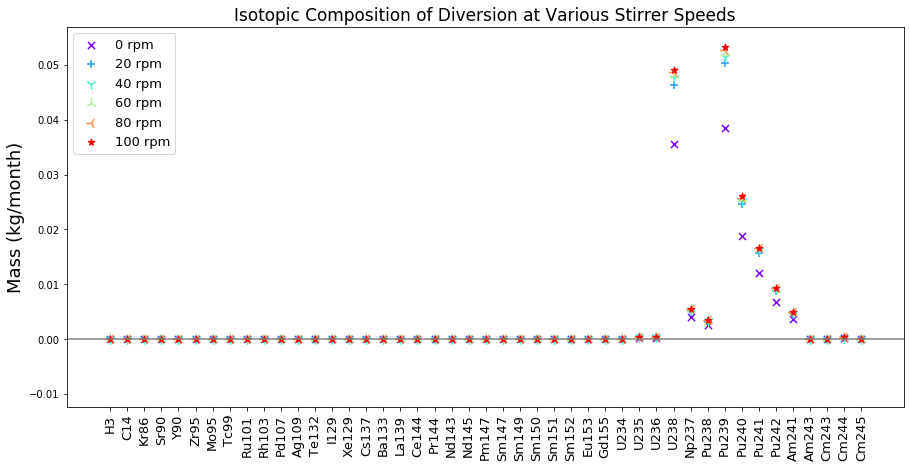
\includegraphics[width=\linewidth]{images/rotation-sa-comp}
	\caption{Isotopic composition of the Diverted material stream at various central stirrer speeds.}
	\label{fig:ref-rot-sa}
\end{figure}

\begin{figure}
	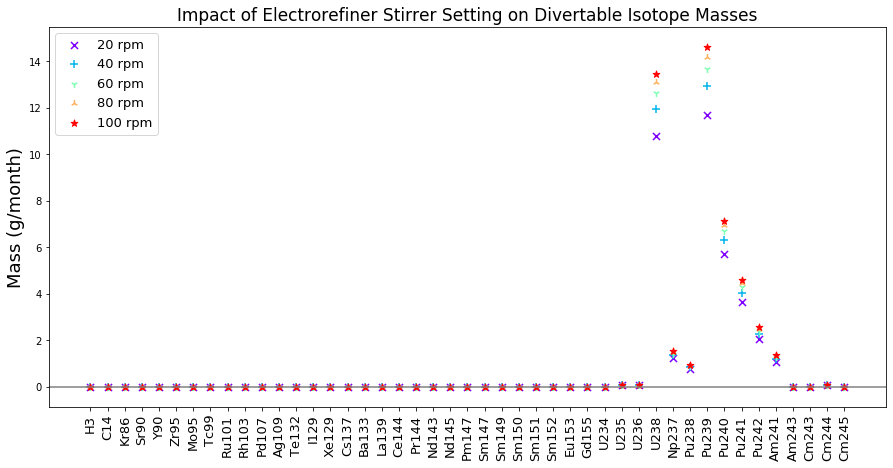
\includegraphics[width=\linewidth]{images/rotation-sa-diff}
	\caption{Isotopic composition of the Diverted material stream at various central stirrer speeds.}
	\label{fig:ref-rot-diff}
\end{figure}

\subsection{Current}

The primary setting for the electrowinning sub-process is the current. An important aspect of
the current's relationship with efficiency is the decrease in separation beginning around 10 A.
This is seen in Figures \ref{fig:win-cur-sa} and \ref{fig:win-cur-diff} as 10 A is close to the efficiency of 5 A. This relationship occurs due to increasing voltage no longer aiding in separation of some lanthanides as described in chapter 2. Figure \ref{fig:win-cur-diff} shows that the key operating range lies within 6-8 A.

\begin{figure}
	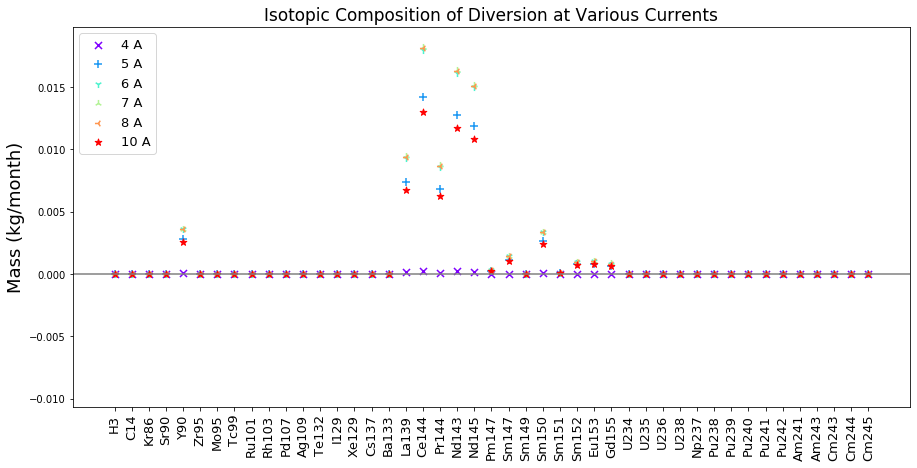
\includegraphics[width=\linewidth]{images/current-sa-comp}
	\caption{Isotopic composition of the Diverted material stream at various Electrowinner currents.}
	\label{fig:win-cur-sa}
\end{figure}

\begin{figure}
	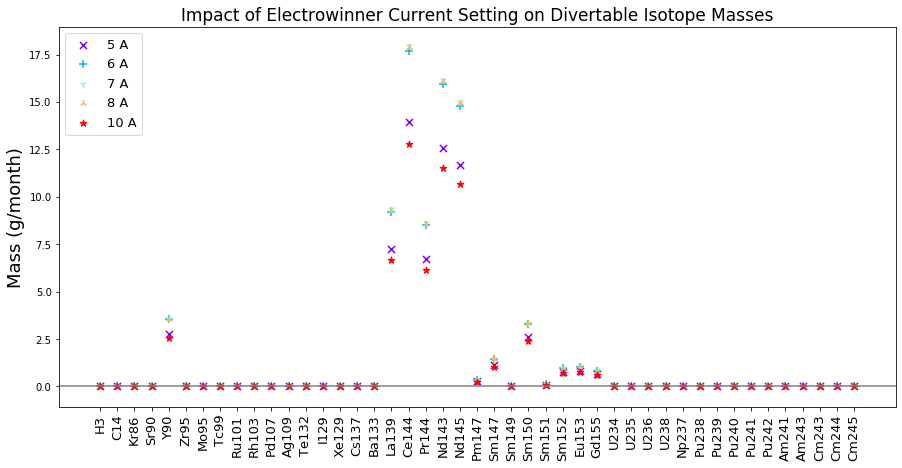
\includegraphics[width=\linewidth]{images/current-sa-diff}
	\caption{Isotopic composition of the Diverted material stream at various Electrowinner currents.}
	\label{fig:win-cur-diff}
\end{figure}

\subsection{Flowrate}

Similar to the central stirrer of the electrorefiner, increasing the flowrate through the electrowinner can aid removal of additional lanthanides and TRU. Flowrates shown are linear rates, with the bounds corresponding to minimum and maximum values tested in experimental facilities. Figures \ref{fig:win-flow-sa} and \ref{fig:win-flow-diff} demonstrate a steady increase in removal rates with increasing flow.

\begin{figure}
	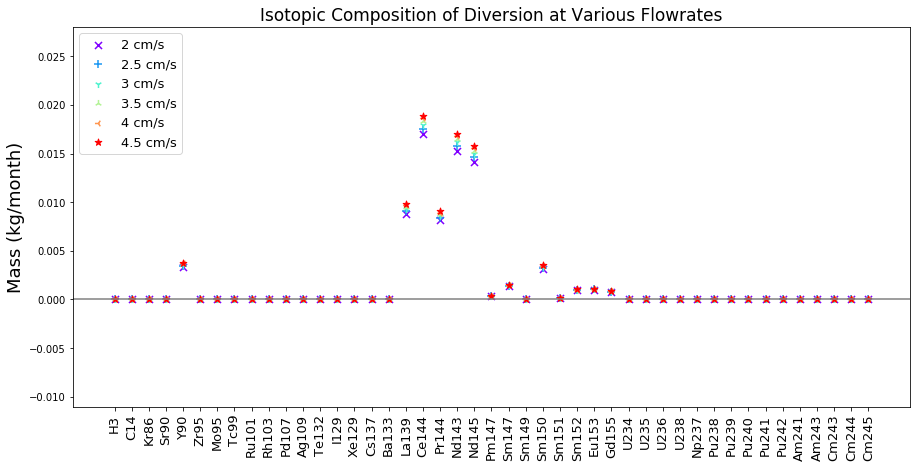
\includegraphics[width=\linewidth]{images/flowrate-sa-comp}
	\caption{Isotopic composition of the Diverted material stream at various Electrowinner flowrates.}
	\label{fig:win-flow-sa}
\end{figure}

\begin{figure}
	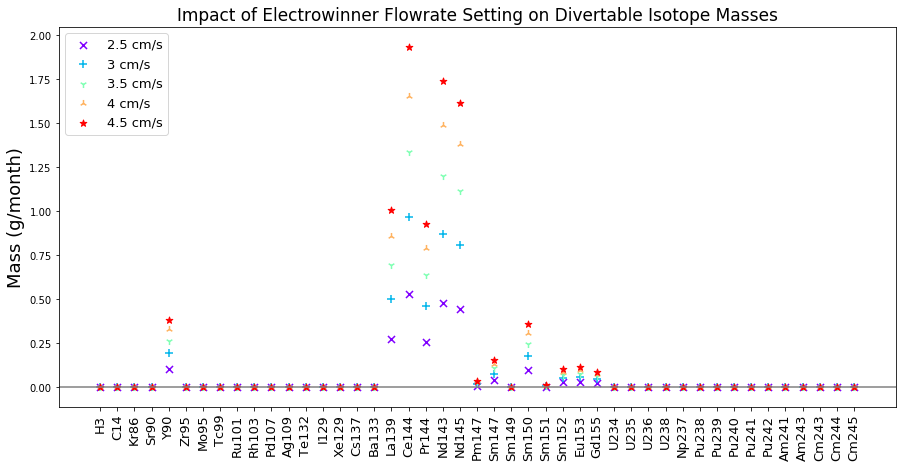
\includegraphics[width=\linewidth]{images/flowrate-sa-diff}
	\caption{Isotopic composition of the Diverted material stream at various Electrowinner flowrates.}
	\label{fig:win-flow-diff}
\end{figure}

\subsection{Reprocessing Time}

The final setting we chose to observe was time spent in the electrowinner. We chose this sub-process since it is closely related to the U/TRU product stream. Comparing Figure \ref{fig:win-time-diff} to Figure \ref{fig:win-flow-diff}, we can see that increasing 
reprocessing time results in more divertable material than the flowrate. 

\begin{figure}
	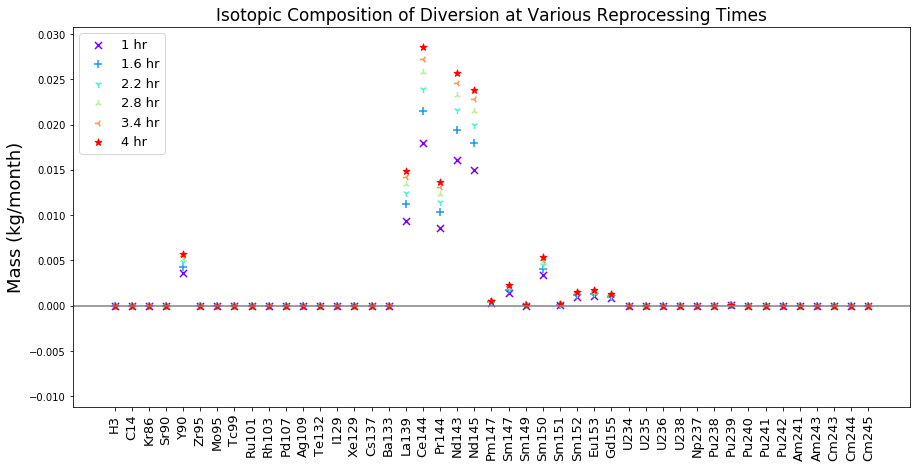
\includegraphics[width=\linewidth]{images/time-sa-comp}
	\caption{Isotopic composition of the Diverted material stream at various Electrowinner reprocessing durations.}
	\label{fig:win-time-sa}
\end{figure}

\begin{figure}
	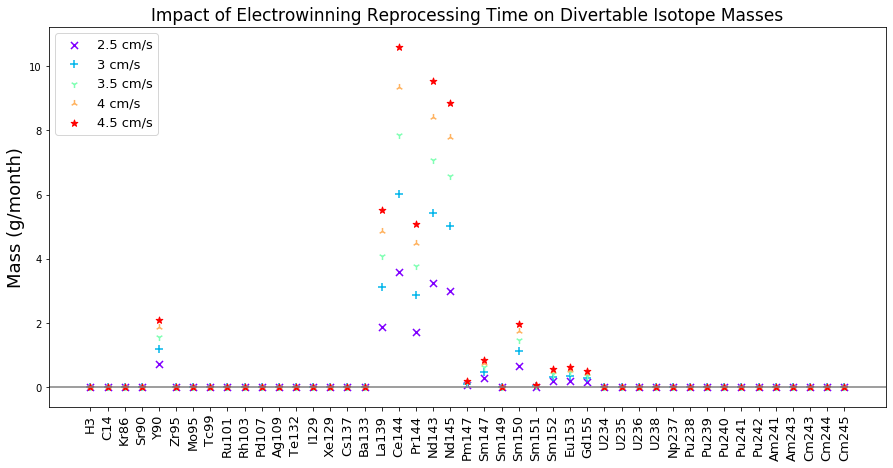
\includegraphics[width=\linewidth]{images/time-sa-diff}
	\caption{Isotopic composition of the Diverted material stream at various Electrowinner reprocessing durations.}
	\label{fig:win-time-diff}
\end{figure}

\section{Parameter Comparison}

The increase due to the previous six operational settings were normalized against their baseline
to determine the most impactful systems. These values are collected in Table \ref{tab:compare}.

\begin{table}[h]
	\centering
	\begin{tabularx}{\linewidth}{lcccccc}
		\hline
		\textbf{Group Number} & \textbf{Temp} & \textbf{Pressure} & \textbf{Stir Speed} & \textbf{Current}
		& \textbf{Flowrate} & \textbf{Time} \\
		\hline \hline
		1 & 0.036 & 8.589 & 30.284 & 5.684 & 3.136 & 20.030 \\ \hline
		2 & 0.715 & 13.336 & 33.542 & 7.216 & 5.699 & 33.602 \\ \hline
		3 & 0.975 & 15.393 & 35.447 & 7.308 & 7.866 & 43.879 \\ 
		4 & 1.672 & 15.912 & 36.799 & 7.281 & 9.743 & 52.154 \\ \hline
		5 & 3.328 & 16.047 & 37.848 & 5.202 & 11.398 & 59.080 \\ \hline
	\end{tabularx}
	\caption {Comparison of Operational Settings' Impact on Divertable Material (shown in
		\% difference).}
	\label {tab:compare}
\end{table}